%%%%%%%%%%%%%%%%%%%%%%%%%%%%%%%%%%%%%
%                                   %
% Compile with XeLaTeX and biber    %
%                                   %
% Questions or comments:            %
%                                   %
% joshua dot mcneill at uga dot edu %
%                                   %
%%%%%%%%%%%%%%%%%%%%%%%%%%%%%%%%%%%%%

\documentclass{beamer}
  % Read in standard preamble (cosmetic stuff)
  %%%%%%%%%%%%%%%%%%%%%%%%%%%%%%%%%%%%%%%%%%%%%%%%%%%%%%%%%%%%%%%%
% This is a standard preamble used in for all slide documents. %
% It basically contains cosmetic settings.                     %
%                                                              %
% Joshua McNeill                                               %
% joshua dot mcneill at uga dot edu                            %
%%%%%%%%%%%%%%%%%%%%%%%%%%%%%%%%%%%%%%%%%%%%%%%%%%%%%%%%%%%%%%%%

% Beamer settings
% \usetheme{Berkeley}
\usetheme{CambridgeUS}
% \usecolortheme{dove}
% \usecolortheme{rose}
\usecolortheme{seagull}
\usefonttheme{professionalfonts}
\usefonttheme{serif}
\setbeamertemplate{bibliography item}{}

% Packages and settings
\usepackage{fontspec}
  \setmainfont{Charis SIL}
\usepackage{hyperref}
  \hypersetup{colorlinks=true,
              allcolors=blue}
\usepackage{graphicx}
  \graphicspath{{../../figures/}}
\usepackage[normalem]{ulem}
\usepackage{enumerate}

% Document information
\author{M. McNeill}
\title[FREN2001]{Français 2001}
\institute{\url{joshua.mcneill@uga.edu}}
\date{}

%% Custom commands
% Lexical items
\newcommand{\lexi}[1]{\textit{#1}}
% Gloss
\newcommand{\gloss}[1]{`#1'}
\newcommand{\tinygloss}[1]{{\tiny`#1'}}
% Orthographic representations
\newcommand{\orth}[1]{$\langle$#1$\rangle$}
% Utterances (pragmatics)
\newcommand{\uttr}[1]{`#1'}
% Sentences (pragmatics)
\newcommand{\sent}[1]{\textit{#1}}
% Base dir for definitions
\newcommand{\defs}{../definitions}


  % Packages and settings

  % Document information
  \subtitle[Émotions et verbes pronominaux]{Les émotions et plus de verbes pronominaux}

\begin{document}
  % Read in the standard intro slides (title page and table of contents)
  \begin{frame}
    \titlepage
    \tiny{Office: % Basically a variable for office hours location
Gilbert 121\\
          Office hours: % Basically a variable for office hours
 lundi, mercredi, vendredi 10:10--11:10
}
  \end{frame}

  \begin{frame}{Quand tu te sens comme ça}
    \begin{columns}
      \column{0.6\textwidth}
        Explique à un/e partenaire quand tu vis \gloss{experience} ces émotions. \\
        \uncover<2->{$\to$ Alors, je suis ...}
        \begin{enumerate}
          \item Je vis \alert{l'anxiété} quand ...
          \item<3->[$\to$] Je suis anxieux/anxieuse.
          \item Je vis \alert{la colère} quand ...
          \item<4->[$\to$] Je suis fâché/e ou furieux/furieuse.
          \item Je vis \alert{la frustration} quand ...
          \item<5->[$\to$] Je suis frustré/e.
          \item Je vis \alert{le bonheur} quand ...
          \item<6->[$\to$] Je suis content/e ou heureux/heureuse ou ravi/e.
        \end{enumerate}
      \column{0.4\textwidth}
        \begin{minipage}[c][0.8\textheight]{\linewidth}
          \begin{center}
            \only<3>{
              
\includegraphics[scale=0.22]{anxieux.jpg}
            }
            \only<4>{
              
\includegraphics[scale=0.2]{fâché.jpg}
            }
            \only<5>{
              \includegraphics[scale=0.18]{frustré.jpg}
            }
            \only<6>{
              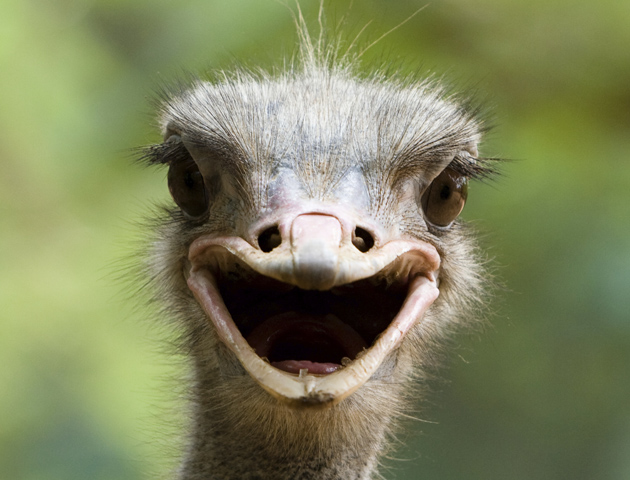
\includegraphics[scale=0.2]{content.jpg}
            }
          \end{center}
        \end{minipage}
    \end{columns}
  \end{frame}

  \begin{frame}{}
    \begin{center}
      \Large Quiz
    \end{center}
  \end{frame}

  \begin{frame}{La maternelle}
    \scriptsize
    \begin{columns}
      \column{0.6\textwidth}
        Christophe explique son expérience à l'école maternelle.
        Complète chaqe description avec un verbe ci-dessous \alert{à l'imparfait}.
        \begin{center}
          \begin{tabular}{| l | l | l |}
            \hline
            s'amuser     & s'ennuyer   & se fâcher \\
            \hline
            se rappeler  & se dépêcher & s'entendre \\
            \hline
            s'occuper de & se reposer  & \\
            \hline
          \end{tabular}
        \end{center}
        \begin{enumerate}
          \item Pendant la récréation, les enfants jouaient ensemble.
          \item<2->[$\to$] Ils s'amusaient.
          \item Après le déjeuner, tout le monde faisait la sieste.
          \item<3->[$\to$] Ils se reposaient.
          \item Jacques et moi, nous étions des bons amis.
          \item<4->[$\to$] Nous nous entendions.
          \item Je n'oubliait jamais les leçons.
          \item<5->[$\to$] Je me rappelais les leçons.
        \end{enumerate}
      \column{0.4\textwidth}
        \begin{center}
          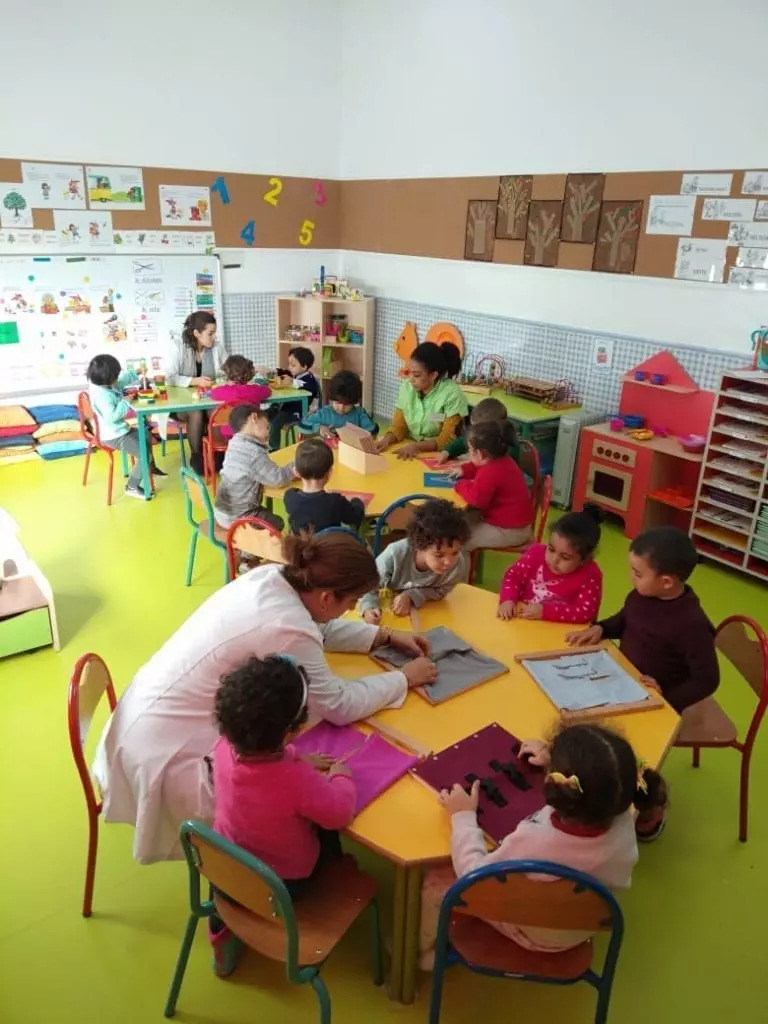
\includegraphics[scale=0.125]{maternelle.jpg}
        \end{center}
    \end{columns}
  \end{frame}

  \begin{frame}{Trouve une personne}
    Trouvez une personne dans la classe pour qui la phrase est vraie et écrivez les noms.
    N'écrivez pas un nom pour plus d'une phrase.
    \begin{description}
      \item[] \textbf{Modèle:} \emph{s'entend bien avec ses parents}
      \item[E1:] Est-ce que \alert{tu t'entends} avec tes parents?
      \item[E2:] Oui, \alert{je m'entends} avec mes parents.
      \item[OU] Non, \alert{je ne m'entends pas} avec mes parents.
    \end{description}
    \vspace{0.25cm}
    Trouve une personne qui...
    \begin{columns}[t]
      \column{0.5\textwidth}
        \begin{enumerate}
          \item s'entend bien avec ses parents.
          \item se rappelle son premier jour à l'école.
          \item s'amuse quelquefois pendant le cours de français.
        \end{enumerate}
      \column{0.5\textwidth}
        \begin{enumerate}
          \setcounter{enumi}{3}
          \item s'occupe toujours du dîner le soir.
          \item s'est dépêchée ce matin.
          \item va se détendre ce weeke-end.
        \end{enumerate}
      \end{columns}
  \end{frame}

  \begin{frame}{}
    \begin{center}
      \Large Questions?
    \end{center}
  \end{frame}
\end{document}
